\documentclass[conference]{IEEEtran}

\usepackage{cite}
\usepackage{amsmath,amssymb}
\usepackage{graphicx}
\usepackage[caption=false,font=footnotesize]{subfig}
\usepackage{algorithm}
\usepackage{algpseudocode}
\usepackage{booktabs}
\usepackage{xcolor}
\usepackage{url}
\usepackage[colorlinks=true,urlcolor=blue,linkcolor=black,citecolor=black]{hyperref}
\usepackage{listings}
\lstset{basicstyle=\ttfamily\tiny,breaklines=true,breakatwhitespace=false,
  columns=fullflexible,keepspaces=true,frame=single}

\newtheorem{definition}{Definition}
\newtheorem{lemma}{Lemma}
\newtheorem{theorem}{Theorem}

\newcommand{\Eq}{\textsc{Eq}}
\newcommand{\cnt}{\mathrm{cnt}}


\begin{document}

\title{Verifying an Election Majority over Equality-Only Ballots: A Divide-and-Conquer Approach}

\author{
\IEEEauthorblockN{Sridhar Kumar}
\IEEEauthorblockA{\textit{Department of Computer Science}\\
\textit{University of Florida}\\
Gainesville, FL, USA\\
f.sridharkumar@ufl.edu}
\and
\IEEEauthorblockN{Daen P Khan}
\IEEEauthorblockA{\textit{Department of Computer Science}\\
\textit{University of Florida}\\
Gainesville, FL, USA\\
dpatan@ufl.edu}
}

\maketitle

\begin{abstract}
Certifying an election requires deciding whether any candidate received more
than half of the ballots. When ballots are encrypted, the tallying authority
may only be able to test whether two ballots are for the same candidate, which
rules out sorting or keeping a tally. We model this task as finding the
majority element of a sequence under an equality oracle and give a
divide-and-conquer algorithm that finds the majority of each half recursively
and then recounts at most two finalists. We prove the algorithm correct and
show that it runs in $O(n\log n)$ time. Experiments on synthetic elections of
up to ten million ballots confirm the predicted growth.
\end{abstract}

\begin{IEEEkeywords}
divide and conquer, majority element, election tallying, encrypted ballots,
equality oracle, recurrence analysis
\end{IEEEkeywords}

%======================================================================
\section{Introduction}
%======================================================================

Many election rules require a candidate to win an \emph{absolute majority},
more than half of all ballots cast, to be declared the winner outright;
otherwise a runoff is held. Deciding whether such a majority exists, and for
whom, is therefore a basic step in certifying a result.

Counting paper ballots is simple. Verifiable voting systems, however, often
keep ballots encrypted during tallying so that no official learns how anyone
voted~\cite{adida2008helios}. Because the encryption is probabilistic, two
ballots for the same candidate look different, so encrypted ballots can be
neither tallied nor sorted. What remains is a \emph{plaintext equivalence
test}~\cite{jakobsson2000mix}, which reveals only whether two ballots are for
the same candidate.

This paper studies how to decide whether an absolute majority exists using only
such equality tests. Our contributions are:
\begin{itemize}
  \item An abstraction of the task as majority finding under an equality
        oracle (Section~\ref{sec:problem}).
  \item A divide-and-conquer algorithm, described formally and as a counting
        procedure (Sections~\ref{sec:algorithm} and~\ref{sec:domain}).
  \item A proof of correctness and an $O(n\log n)$ running-time analysis
        (Sections~\ref{sec:analysis} and~\ref{sec:proof}).
  \item An experimental validation on synthetic elections
        (Section~\ref{sec:experiments}).
\end{itemize}

%======================================================================
\section{Related Work}
%======================================================================

The best-known algorithm for the majority problem is the Boyer--Moore voting
algorithm (MJRTY)~\cite{boyer1991mjrty}. It cancels out pairs of ballots for
different candidates in one pass and verifies the surviving candidate in a
second, using only equality tests and $O(n)$ time. Misra and Gries~\cite{misra1982finding}
generalized this idea to find every value occurring more than $n/k$ times,
which underlies modern streaming ``heavy hitter'' summaries. We use
Boyer--Moore as a baseline; the divide-and-conquer approach is asymptotically
slower but splits naturally into independent sub-tallies, matching how ballots
are divided among counting teams.

On the voting side, Helios~\cite{adida2008helios} is a deployed web-based
voting system that keeps ballots encrypted and lets anyone audit the tally.
The plaintext equivalence test of Jakobsson and Juels~\cite{jakobsson2000mix}
lets parties holding a decryption key jointly decide whether two ciphertexts
encrypt the same message without revealing the message, which is exactly the
equality oracle in our model.

Our analysis uses standard tools for divide-and-conquer
algorithms~\cite{cormen2009introduction}, in particular the Master Theorem for
recurrences of the form $T(n) = aT(n/b) + f(n)$, introduced in general form by
Bentley, Haken, and Saxe~\cite{bentley1980general}.

%======================================================================
\section{Problem Formulation}\label{sec:problem}
%======================================================================

\subsection{Real-World Context}

An election authority holds $n$ encrypted ballots, each cast for one of an
unknown number of candidates. The authority must certify either that some
candidate received more than $n/2$ ballots, and which one, or that no candidate
did and a runoff is needed. Each comparison of two ballots is a cryptographic
protocol run jointly by the trustees, so it is the expensive operation; the
authority wants to use as few comparisons as possible and to split the work
among several counting teams.

\subsection{Mathematical Abstraction}

\begin{definition}[Ballot sequence]
Let $U$ be a set of possible ballot values (candidates), whose size need not
be known. A ballot sequence is $B = (b_0, b_1, \ldots, b_{n-1})$ with each
$b_i \in U$. For indices $0 \le lo < hi \le n$ we write $B[lo..hi)$ for the
contiguous subsequence $(b_{lo}, \ldots, b_{hi-1})$, of length $hi - lo$.
\end{definition}

\begin{definition}[Equality oracle]
The only operation on ballot values is
$\Eq : U \times U \to \{\text{true}, \text{false}\}$, with
$\Eq(x, y) = \text{true}$ if and only if $x = y$. There is no order on $U$ and
no way to map a value to an index or hash, so sorting and tally tables are
unavailable.
\end{definition}

\begin{definition}[Count and majority]
For a sequence $S$ and a value $x$, let $\cnt_S(x)$ be the number of positions
of $S$ holding $x$. A value $x$ is the \emph{majority} of $S$ if
$\cnt_S(x) > |S|/2$.
\end{definition}

A sequence has at most one majority: two distinct majorities would together
occupy more than $|S|$ positions. Since $\cnt_S(x)$ is an integer,
$\cnt_S(x) > |S|/2$ holds exactly when $\cnt_S(x) > \lfloor |S|/2 \rfloor$.

\medskip
\noindent\textbf{Problem (Majority Verification).}
\emph{Input:} a ballot sequence $B$ of length $n \ge 1$, accessible only
through $\Eq$.
\emph{Output:} the majority of $B$ if one exists, and the symbol $\bot$
(``no majority'') otherwise.
\emph{Cost:} the number of calls to $\Eq$, together with the running time.

\medskip
\noindent\textbf{Tree view.} Recursively halving $B$ produces a full binary
tree whose root is $B$, whose internal nodes are contiguous segments
$B[lo..hi)$ of length at least $2$, and whose $n$ leaves are the single
ballots. Each internal node has two children, the left and right halves of its
segment, so the tree has exactly $n - 1$ internal nodes. The algorithm below
computes, bottom-up, the majority (or $\bot$) of every node of this tree.

%======================================================================
\section{Algorithm Design}\label{sec:algorithm}
%======================================================================

\subsection{Divide-and-Conquer Strategy}

The algorithm rests on one observation, proved as Lemma~\ref{lem:split}: if a
candidate is the majority of a sequence, it must be the majority of at least
one of the two halves. Therefore, once the majority of each half is known,
the only possible majority of the whole is one of those two values, and
checking each of them takes a single pass. Algorithm~\ref{alg:dc} implements
the three steps:
\begin{itemize}
  \item \textbf{Divide:} split $B[lo..hi)$ at $mid = \lfloor (lo+hi)/2 \rfloor$.
  \item \textbf{Conquer:} recursively compute the majority $\ell$ of the left
        half and $r$ of the right half (each possibly $\bot$).
  \item \textbf{Combine:} if both are $\bot$, return $\bot$; if both exist and
        are equal, return that value; otherwise count each existing finalist
        over the whole segment and return the one, if any, that exceeds half.
\end{itemize}
A finalist is carried as a representative ballot from its half, so comparing
two finalists, or a finalist against a ballot, is itself one call to $\Eq$.

\begin{algorithm}[t]
\caption{Divide-and-conquer majority verification}
\label{alg:dc}
\begin{algorithmic}[1]
\Require ballot sequence $B$, indices $0 \le lo < hi \le |B|$
\Ensure majority of $B[lo..hi)$, or $\bot$ if none exists
\Function{MajorityDC}{$B, lo, hi$}
  \If{$hi - lo = 1$}
    \State \Return $b_{lo}$ \Comment{base case}
  \EndIf
  \State $mid \gets \lfloor (lo + hi)/2 \rfloor$ \Comment{divide}
  \State $\ell \gets$ \Call{MajorityDC}{$B, lo, mid$} \Comment{conquer}
  \State $r \gets$ \Call{MajorityDC}{$B, mid, hi$}
  \If{$\ell = \bot$ \textbf{and} $r = \bot$} \Comment{combine}
    \State \Return $\bot$
  \EndIf
  \If{$\ell \ne \bot$ \textbf{and} $r \ne \bot$ \textbf{and} $\Eq(\ell, r)$}
    \State \Return $\ell$
  \EndIf
  \For{each $x \in (\ell, r)$ with $x \ne \bot$}
    \If{\Call{Count}{$B, lo, hi, x$} $> \lfloor (hi - lo)/2 \rfloor$}
      \State \Return $x$
    \EndIf
  \EndFor
  \State \Return $\bot$
\EndFunction
\Statex
\Function{Count}{$B, lo, hi, x$}
  \State $c \gets 0$
  \For{$i \gets lo$ \textbf{to} $hi - 1$}
    \If{$\Eq(b_i, x)$}
      \State $c \gets c + 1$
    \EndIf
  \EndFor
  \State \Return $c$
\EndFunction
\end{algorithmic}
\end{algorithm}

The full problem is solved by the call \textsc{MajorityDC}$(B, 0, n)$.

\subsection{Worked Example}

Consider eight ballots $B = (A, A, B, A \mid B, A, C, A)$.
\begin{itemize}
  \item Left half $(A, A, B, A)$: its halves $(A, A)$ and $(B, A)$ return
        $A$ and $\bot$, and recounting $A$ gives $3 > 2$, so the left half
        returns $A$.
  \item Right half $(B, A, C, A)$: its halves $(B, A)$ and $(C, A)$ both
        return $\bot$, so the right half returns $\bot$ without any counting.
  \item Root: the finalists are $A$ and $\bot$. Recounting $A$ over all eight
        ballots gives $5 > 4$, so the algorithm returns $A$.
\end{itemize}

\subsection{Implementation Notes}

The recursion works on index ranges of the original array, so no ballots are
copied. In our Java implementation (see Code Availability), each ballot is
stored as an integer, but every inspection of ballot values goes through a
single method \texttt{same(a, b)} that performs one equality test and
increments a counter. This keeps the implementation faithful to the
equality-only model and lets the experiments report the exact number of
oracle calls.

%======================================================================
\section{Complexity Analysis}\label{sec:analysis}
%======================================================================

\subsection{Number of Equality Tests}

\begin{theorem}\label{thm:bound}
On $n \ge 2$ ballots, \textsc{MajorityDC} makes at most
$2n\lceil\log_2 n\rceil + n - 1$ calls to $\Eq$.
\end{theorem}

\begin{IEEEproof}
Leaves (single ballots) make no calls. Consider an internal node of the
recursion tree whose segment has length $s \ge 2$. Its combine step makes at
most one call comparing $\ell$ with $r$, and at most two calls to
\textsc{Count}, each making exactly $s$ calls. So the node makes at most
$2s + 1$ calls. The tree has $n - 1$ internal nodes, contributing at most
$n - 1$ in total for the ``$+1$'' terms.

For the $2s$ terms, group internal nodes by depth. The segments at any one
depth are disjoint pieces of $B$, so their lengths sum to at most $n$. A node
at depth $d$ has length at most $\lceil n / 2^d \rceil$, and an internal node
has length at least $2$; since $\lceil n/2^d \rceil \ge 2$ requires
$2^d < n$, internal nodes occur only at depths
$0, 1, \ldots, \lceil\log_2 n\rceil - 1$, which is $\lceil \log_2 n\rceil$
depths. Summing $2s$ over these depths gives at most
$2n\lceil\log_2 n\rceil$. Adding the two parts proves the bound.
\end{IEEEproof}

\subsection{Running Time}

Let $T(n)$ be the worst-case running time on $n$ ballots. The divide step
takes constant time, the two recursive calls are on
$\lfloor n/2 \rfloor$ and $\lceil n/2 \rceil$ ballots, and the combine step
takes at most two linear scans. Hence, for a constant $c > 0$,
\begin{equation}
T(n) \le T(\lceil n/2 \rceil) + T(\lfloor n/2 \rfloor) + c\,n,
\qquad T(1) = O(1).
\label{eq:recurrence}
\end{equation}
Ignoring floors and ceilings, which does not affect the asymptotic
solution~\cite{cormen2009introduction}, this is $T(n) = aT(n/b) + f(n)$ with
$a = 2$, $b = 2$, and $f(n) = \Theta(n)$. Since
$n^{\log_b a} = n^{\log_2 2} = n$ and $f(n) = \Theta(n^{\log_b a})$, Case~2
of the Master Theorem~\cite{bentley1980general,cormen2009introduction} gives
\begin{equation}
T(n) = O(n \log n).
\label{eq:nlogn}
\end{equation}
This agrees with Theorem~\ref{thm:bound}, since the work per call is
proportional to the number of equality tests plus a constant.

The bound is an upper bound on the worst case; some inputs are cheaper. If all
ballots are identical, every combine step makes a single agreement test, so
the total is $n - 1$ tests and $\Theta(n)$ time. Likewise, when a candidate
holds a large share, halves usually agree and recounts become rare, and when
no candidate is close to half, halves usually both return $\bot$ and stop
immediately. Section~\ref{sec:experiments} observes both effects.

\subsection{Space}

The algorithm needs no auxiliary arrays. The recursion depth is
$\lceil\log_2 n\rceil$, and each stack frame stores a constant number of
indices and finalists, so the extra space is $O(\log n)$ beyond the $O(n)$
input.

%======================================================================
\section{Proof of Correctness}\label{sec:proof}
%======================================================================

Throughout, let $S = L \circ R$ denote a sequence $S$ split into a left part
$L$ and a right part $R$, so that $|S| = |L| + |R|$ and
$\cnt_S(x) = \cnt_L(x) + \cnt_R(x)$ for every value $x$.

\begin{lemma}[Majority split]\label{lem:split}
If $x$ is the majority of $S = L \circ R$, then $x$ is the majority of $L$ or
the majority of $R$ (or both).
\end{lemma}

\begin{IEEEproof}
Suppose, for contradiction, that $x$ is the majority of neither part. Then
$\cnt_L(x) \le |L|/2$ and $\cnt_R(x) \le |R|/2$, so
$\cnt_S(x) = \cnt_L(x) + \cnt_R(x) \le (|L| + |R|)/2 = |S|/2$,
contradicting that $x$ is the majority of $S$.
\end{IEEEproof}

\begin{lemma}[Agreement]\label{lem:agree}
If $x$ is the majority of both $L$ and $R$, then $x$ is the majority of
$S = L \circ R$.
\end{lemma}

\begin{IEEEproof}
$\cnt_S(x) = \cnt_L(x) + \cnt_R(x) > |L|/2 + |R|/2 = |S|/2$.
\end{IEEEproof}

\begin{theorem}\label{thm:correct}
For every ballot sequence $B$ and indices $0 \le lo < hi \le |B|$,
\textsc{MajorityDC}$(B, lo, hi)$ terminates and returns the majority of
$B[lo..hi)$ if one exists, and $\bot$ otherwise.
\end{theorem}

\begin{IEEEproof}
We use strong induction on the segment length $m = hi - lo \ge 1$. Write
$S = B[lo..hi)$, $L = B[lo..mid)$, and $R = B[mid..hi)$.

\emph{Base case ($m = 1$).} The single ballot $b_{lo}$ appears $1 > 1/2$
times, so it is the majority of $S$, and the algorithm returns it.

\emph{Inductive step ($m \ge 2$).} Assume the claim holds for all lengths
smaller than $m$. Since $m \ge 2$, both $|L| = \lfloor m/2 \rfloor$ and
$|R| = \lceil m/2 \rceil$ are at least $1$ and at most $m - 1$. By the
induction hypothesis, both recursive calls terminate, $\ell$ is the majority
of $L$ or $\bot$ if $L$ has none, and $r$ is the majority of $R$ or $\bot$ if
$R$ has none. We consider the three ways the combine step can end.

\emph{Case 1: $\ell = r = \bot$.} Neither half has a majority, so by
Lemma~\ref{lem:split} no value is the majority of $S$. Returning $\bot$ is
correct.

\emph{Case 2: $\ell \ne \bot$, $r \ne \bot$, and $\ell = r$.} The value
$\ell$ is the majority of both halves, so by Lemma~\ref{lem:agree} it is the
majority of $S$. Returning $\ell$ is correct.

\emph{Case 3: otherwise.} Let $K$ be the set of non-$\bot$ values among
$\ell$ and $r$; it is nonempty and has at most two elements. By
Lemma~\ref{lem:split}, every majority of $S$ is the majority of $L$ or of
$R$, so it lies in $K$. For each $x \in K$, \textsc{Count} examines every
position of $S$ once and returns exactly $\cnt_S(x)$, and the test
$\cnt_S(x) > \lfloor m/2 \rfloor$ holds exactly when $x$ is the majority of
$S$. If $S$ has a majority, it is in $K$ and passes the test, and since the
majority is unique, no other value in $K$ can pass, so the algorithm returns
it. If $S$ has no majority, no value in $K$ passes, and the algorithm returns
$\bot$. In both situations the result is correct.

The combine step performs at most two loops of $m$ iterations, so the call
terminates. This completes the induction; taking $lo = 0$ and $hi = n$ shows
that \textsc{MajorityDC}$(B, 0, n)$ solves Majority Verification.
\end{IEEEproof}

%======================================================================
\section{The Algorithm as an Election Procedure}\label{sec:domain}
%======================================================================

In the language of the election, the algorithm is a hierarchical counting
procedure that never reveals more than ``same candidate or not'' about any
pair of ballots.

The chief election official splits the stack of sealed ballots into two
roughly equal piles and hands each pile to a counting team. Each team splits
its pile again and delegates, until every pile holds a single ballot, whose
``leader'' is simply the candidate on it. Teams then report upward. Each team
receives two reports, one from each sub-team, stating either a provisional
leader of that sub-pile (represented by one of its ballots) or ``no
leader.''
\begin{itemize}
  \item If \textbf{both sub-teams report no leader}, the team reports no
        leader without examining anything: a candidate who failed to reach
        half of both sub-piles cannot reach half of the combined pile.
  \item If \textbf{both report the same leader}, confirmed by one equivalence
        test between their representative ballots, that candidate leads the
        combined pile: more than half of each sub-pile adds up to more than
        half of the whole.
  \item Otherwise, at most two \textbf{finalists} remain. The team runs a
        recount, comparing each finalist's representative ballot against
        every ballot in its pile, and reports whichever finalist exceeds half,
        or no leader.
\end{itemize}
The chief official's final report is the certified outcome: either the
candidate holding an absolute majority, or the conclusion that a runoff is
required. No candidate can be overlooked, because a true majority winner
always survives as a finalist in at least one sub-pile at every level. Teams
at the same level work on disjoint piles and never need to coordinate, so the
procedure parallelizes naturally across counting rooms or precincts.

%======================================================================
\section{Experimental Validation}\label{sec:experiments}
%======================================================================

\begin{figure*}[!t]
\centering
\subfloat[Running time on \textsc{Tie} elections (median of five trials; bars
show minimum and maximum) with the least-squares fit $c\,n\log_2 n$,
$c \approx 0.94$~ns.\label{fig:fit}]{%
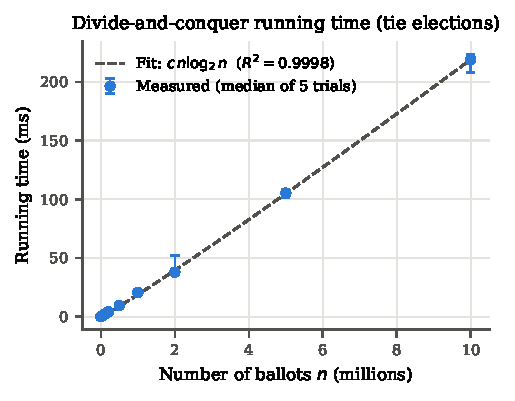
\includegraphics[width=0.48\textwidth]{figures/fig1_runtime_fit.pdf}}
\hfill
\subfloat[Running time divided by $n\log_2 n$. A flat curve indicates
$\Theta(n\log n)$ growth.\label{fig:normalized}]{%
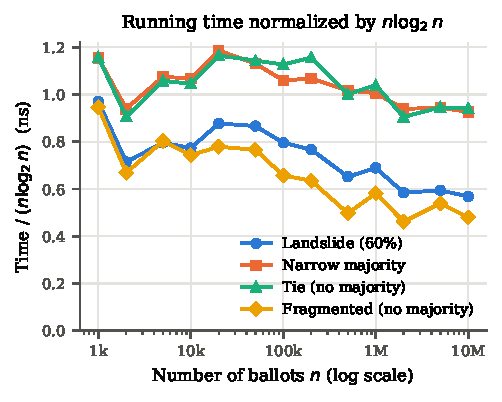
\includegraphics[width=0.48\textwidth]{figures/fig2_normalized_time.pdf}}
\\[4pt]
\subfloat[Equality tests divided by $n\log_2 n$, with the bound of
Theorem~\ref{thm:bound} (dashed).\label{fig:comparisons}]{%
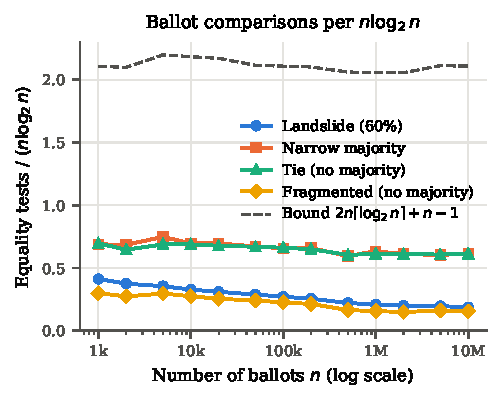
\includegraphics[width=0.48\textwidth]{figures/fig3_comparisons.pdf}}
\hfill
\subfloat[Running time of the three methods on \textsc{Tie} elections
(log--log scale).\label{fig:baselines}]{%
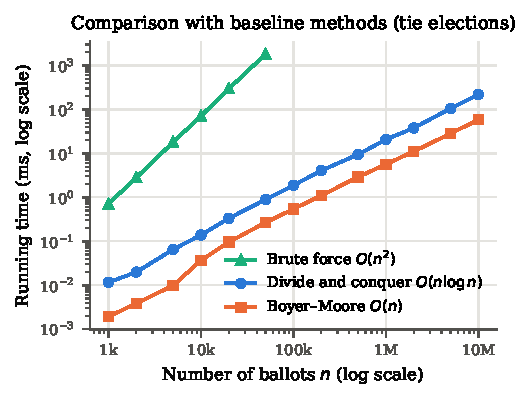
\includegraphics[width=0.48\textwidth]{figures/fig4_baselines.pdf}}
\caption{Experimental results for \textsc{MajorityDC} on synthetic elections
of $10^3$ to $10^7$ ballots.}
\label{fig:results}
\end{figure*}

\subsection{Implementation and Correctness Testing}

We implemented Algorithm~\ref{alg:dc} in Java, together with two baselines
used for testing and comparison: a brute-force method that recounts every
ballot's candidate ($O(n^2)$), and the Boyer--Moore voting
algorithm~\cite{boyer1991mjrty} ($O(n)$). Before timing, we checked that the three
methods agree on 210{,}160 inputs, including every sequence of length up to 8
over three candidates. All tests passed, and no run exceeded the bound of
Theorem~\ref{thm:bound}.

\subsection{Synthetic Elections and Setup}

Each synthetic election has five candidates and randomly shuffled ballots
(Table~\ref{tab:scenarios}). \textsc{Tie} and \textsc{Narrow} are the hardest
cases, since the leader holds about half of every large sub-pile.

\begin{table}[t]
\centering
\caption{Synthetic election scenarios (five candidates)}
\label{tab:scenarios}
\begin{tabular}{@{}lll@{}}
\toprule
Scenario & Candidate 0 receives & Outcome \\
\midrule
\textsc{Landslide}  & $\lfloor 0.6n \rfloor$ ballots & 0 wins \\
\textsc{Narrow}     & $\lfloor n/2 \rfloor + 1$ ballots & 0 wins by one \\
\textsc{Tie}        & $\lfloor n/2 \rfloor$ ballots & no majority \\
\textsc{Fragmented} & about $n/5$ (uniform) & no majority \\
\bottomrule
\end{tabular}
\end{table}

We tested thirteen sizes from $n = 10^3$ to $10^7$, with five random trials
per size and scenario (brute force only up to $5\cdot 10^4$). After a JVM
warm-up, each trial was repeated until at least 20~ms had elapsed, and we
report the median of the five trials. Experiments ran on a two-vCPU Linux
virtual machine with OpenJDK~21.
% TODO: if you re-run the experiments on your own computer, replace the
% hardware description above and regenerate the figures.

\subsection{Results}


\begin{table}[t]
\centering
\caption{Median running time of \textsc{MajorityDC} (ms)}
\label{tab:results}
\begin{tabular}{@{}rrrrr@{}}
\toprule
$n$ & \textsc{Landslide} & \textsc{Narrow} & \textsc{Tie} & \textsc{Fragm.} \\
\midrule
$10^3$ & 0.010 & 0.012 & 0.012 & 0.009 \\
$10^4$ & 0.103 & 0.142 & 0.139 & 0.099 \\
$10^5$ & 1.322 & 1.760 & 1.873 & 1.092 \\
$10^6$ & 13.745 & 20.057 & 20.733 & 11.602 \\
$10^7$ & 132.161 & 215.525 & 218.795 & 111.619 \\
\bottomrule
\end{tabular}
\end{table}

\textbf{Running time matches $n\log n$.} On the worst-case \textsc{Tie} elections,
a fitted $c\,n\log_2 n$ curve explains the measured times with $R^2 = 0.9998$
(Fig.~\ref{fig:fit}); ten million ballots take about 219~ms
(Table~\ref{tab:results}).

\textbf{Normalized time is nearly constant.} Divided by $n\log_2 n$, the running
time for \textsc{Narrow} and \textsc{Tie} stays between about $0.9$ and
$1.2$~ns across four orders of magnitude (Fig.~\ref{fig:normalized}).
\textsc{Landslide} and \textsc{Fragmented} elections fall below this level, as
predicted in Section~\ref{sec:analysis}, because their halves usually agree or
both report no leader, so fewer recounts are needed.

\textbf{Equality tests stay within the bound.} For \textsc{Tie} elections the
algorithm uses about $0.6$--$0.7\,n\log_2 n$ equality tests, roughly 30\% of
the proven bound, and no trial exceeded it (Fig.~\ref{fig:comparisons}).
Unlike running time, this count does not depend on the machine.

\textbf{Comparison with baselines.} Brute force grows
quadratically and takes about 1.8~s at $n = 5\cdot 10^4$, versus 0.89~ms for
divide and conquer; Boyer--Moore is about $3.8\times$ faster at $n = 10^7$
(Fig.~\ref{fig:baselines}).

%======================================================================
\section{Discussion}
%======================================================================

\subsection{When Divide and Conquer Fits}

For a purely sequential tally, Boyer--Moore is faster. The
divide-and-conquer algorithm's strengths are structural: its recursive calls
are independent, so sub-piles can be verified by separate teams or processors,
and every intermediate report states the majority of a specific pile, which
supports auditing at the level of individual counting rooms.

\subsection{Limitations}

The experiments use synthetic, uniformly shuffled ballots; real ballot
orders may be correlated with precinct, which can change how often recounts
occur but not the worst-case bound. Running times are machine-dependent, and
we model the equality test as a unit-cost operation rather than implementing
the cryptographic protocol.

%======================================================================
\section{Conclusion}
%======================================================================

We gave a divide-and-conquer algorithm for verifying an election majority
when ballots can only be compared for equality, based on the fact that a
majority of the whole must be a majority of one of its halves. We proved it
correct, showed that it runs in $O(n\log n)$ time, and confirmed the analysis
experimentally. Future work includes a parallel implementation and an
evaluation with a real plaintext equivalence test.

%======================================================================
\begin{thebibliography}{9}

\bibitem{adida2008helios}
B.~Adida, ``Helios: Web-based open-audit voting,'' in \emph{Proc. 17th USENIX
Security Symposium}, San Jose, CA, USA, 2008.

\bibitem{jakobsson2000mix}
M.~Jakobsson and A.~Juels, ``Mix and match: Secure function evaluation via
ciphertexts,'' in \emph{Advances in Cryptology -- ASIACRYPT 2000}, ser. Lecture
Notes in Computer Science, vol. 1976. Berlin, Germany: Springer, 2000,
pp. 162--177.

\bibitem{boyer1991mjrty}
R.~S. Boyer and J.~S. Moore, ``MJRTY---A fast majority vote algorithm,'' in
\emph{Automated Reasoning: Essays in Honor of Woody Bledsoe}, R.~S. Boyer, Ed.
Dordrecht, The Netherlands: Kluwer Academic Publishers, 1991, pp. 105--117.

\bibitem{misra1982finding}
J.~Misra and D.~Gries, ``Finding repeated elements,'' \emph{Science of
Computer Programming}, vol.~2, no.~2, pp. 143--152, 1982.

\bibitem{cormen2009introduction}
T.~H. Cormen, C.~E. Leiserson, R.~L. Rivest, and C.~Stein, \emph{Introduction
to Algorithms}, 3rd~ed. Cambridge, MA, USA: MIT Press, 2009.

\bibitem{bentley1980general}
J.~L. Bentley, D.~Haken, and J.~B. Saxe, ``A general method for solving
divide-and-conquer recurrences,'' \emph{ACM SIGACT News}, vol.~12, no.~3,
pp. 36--44, 1980.

\end{thebibliography}

\appendices

\section{Runtime Validation Code}

The following Java source files perform correctness checks, generate the
synthetic elections, measure repeated timing trials, and write the CSV data
used for the experimental figures.  The majority algorithm is included
because it is the implementation called by the benchmark.

\lstinputlisting[language=Java,caption={Divide-and-conquer benchmark and validation harness}]{Benchmark.java}
\lstinputlisting[language=Java,caption={Majority algorithm implementation}]{MajorityVote.java}

\section{LLM Usage}\label{app:llm}

\subsection{Tool and Scope}

We used Claude (model Claude Opus 5.5, by Anthropic), accessed through the
claude.ai web interface in October 2026. It was used to tackle the correctness of the problem,
implement some of the Java code and plotting script, run the experiments, generate the
figures, draft this report in LaTeX.

\subsection{Prompts and Outputs}


The LLM was asked in prompts to question the correctness of certain concepts. The prompts have been cleaned up but essentially they boil down to the following

\begin{enumerate}
\item \textbf{Question:} \emph{Prove that if $x$ is the majority of
$L \circ R$, then $x$ is the majority of $L$ or of $R$. Make sure it holds
when $|L| \ne |R|$.}\\
\textbf{Answer:} Suppose $x$ is the majority of neither part. Then
$\cnt_L(x) \le |L|/2$ and $\cnt_R(x) \le |R|/2$, and adding gives
$\cnt_S(x) \le |S|/2$, a contradiction. The argument never uses $|L| = |R|$,
so it holds for every split, including the $\lfloor m/2 \rfloor$ /
$\lceil m/2 \rceil$ split used for odd $m$.

\item \textbf{Question:} \emph{Show that a sequence has at most one majority,
and that $\cnt > m/2$ is equivalent to $\cnt > \lfloor m/2 \rfloor$ for
integer counts.}\\
\textbf{Answer:} Two distinct values occupy disjoint positions, so
$\cnt_S(x) + \cnt_S(y) \le |S|$; if both exceeded $|S|/2$ the sum would exceed
$|S|$. For the threshold, the two conditions coincide when $m$ is even. When
$m$ is odd, $m/2 = \lfloor m/2 \rfloor + \tfrac12$, and an integer $c$
satisfies $c > \lfloor m/2 \rfloor + \tfrac12$ exactly when
$c \ge \lfloor m/2 \rfloor + 1$, that is, when $c > \lfloor m/2 \rfloor$.

\item \textbf{Question:} \emph{Is the case split on $(\ell, r)$ in
Theorem~\ref{thm:correct} exhaustive?}\\
\textbf{Answer:} Yes. Each of $\ell, r$ is either $\bot$ or a value, giving
four combinations: both $\bot$ (Case~1); both values and equal (Case~2); both
values and distinct (Case~3); exactly one $\bot$ (Case~3). Because $\Eq$ is an
exact equality test, the algorithm's condition $\Eq(\ell, r)$ matches the
proof's condition $\ell = r$.

\item \textbf{Question:} \emph{In Case~3 with $\ell \ne r$ and both existing,
can both finalists pass the count test?}\\
\textbf{Answer:} No. Passing the test means $\cnt_S(x) > \lfloor m/2 \rfloor$,
which by the previous answer means $x$ is the majority of $S$, and a sequence
has at most one majority. Hence the order in which the loop checks the
finalists does not affect the result.

\item \textbf{Question:} \emph{Is the case $\ell = \bot$, $r \ne \bot$ fully
covered by the recount branch?}\\
\textbf{Answer:} Yes. Here $K = \{r\}$. Since $L$ has no majority,
Lemma~\ref{lem:split} implies that any majority of $S$ must be the majority
of $R$, which is $r$. The algorithm counts $r$ over $S$ and returns it exactly
when it exceeds $\lfloor m/2 \rfloor$, and returns $\bot$ otherwise; both
outcomes are correct. The loop skips $\bot$, so no equality test is made on
it. The case $\ell \ne \bot$, $r = \bot$ is symmetric.

\item \textbf{Question:} \emph{Where exactly does the proof use $m \ge 2$?}\\
\textbf{Answer:} Since $mid = \lfloor (lo+hi)/2 \rfloor$ and $lo$ is an
integer, $|L| = mid - lo = \lfloor m/2 \rfloor$ and
$|R| = \lceil m/2 \rceil$. For $m \ge 2$ we get $\lfloor m/2 \rfloor \ge 1$
and $\lceil m/2 \rceil \le m - 1$, so both halves are non-empty (the
recursive calls satisfy the precondition $lo < hi$) and strictly shorter
than $m$ (the induction hypothesis applies). For $m = 1$ one half would be
empty, which is why $m = 1$ is the base case.

\item \textbf{Question:} \emph{Prove an exact upper bound on the number of
equality tests by counting the internal nodes of the recursion tree and
bounding the work per level.}\\
\textbf{Answer:} An internal node with segment length $s$ makes at most one
agreement test and at most two counts of $s$ tests each, so at most $2s + 1$
tests. The recursion tree is a full binary tree with $n$ leaves, so it has
$n - 1$ internal nodes, contributing at most $n - 1$ for the ``$+1$'' terms.
Segments at the same depth are disjoint, so their lengths sum to at most $n$,
and internal nodes occur at $\lceil \log_2 n \rceil$ depths (next answer).
The total is at most $2n\lceil\log_2 n\rceil + n - 1$, as in
Theorem~\ref{thm:bound}.

\item \textbf{Question:} \emph{Justify that internal nodes occur at only
$\lceil \log_2 n \rceil$ depths when $n$ is not a power of~2.}\\
\textbf{Answer:} By induction on depth, a node at depth $d$ has length at
most $\lceil n/2^d \rceil$, using $\lceil \lceil a \rceil / 2 \rceil =
\lceil a/2 \rceil$. An internal node has length at least $2$, and
$\lceil n/2^d \rceil \ge 2$ holds exactly when $2^d < n$, that is, when
$d \le \lceil \log_2 n \rceil - 1$. For example, with $n = 5$ the internal
nodes have lengths $5$ (depth~0), $2$ and $3$ (depth~1), and $2$ (depth~2),
which is $\lceil \log_2 5 \rceil = 3$ depths.

\item \textbf{Question:} \emph{Is applying the Master Theorem valid with
floors and ceilings?}\\
\textbf{Answer:} Yes; Section~4.6.2 of~\cite{cormen2009introduction} shows
that the Master Theorem's conclusions still hold when the subproblem sizes are
$\lfloor n/b \rfloor$ or $\lceil n/b \rceil$. A direct argument also avoids
the issue: by Theorem~\ref{thm:bound} the algorithm makes at most
$2n\lceil\log_2 n\rceil + n - 1$ equality tests, and each of its $2n - 1$
recursive calls does $O(1)$ work besides those tests, so
$T(n) = O(n \log n)$.
\end{enumerate}

\subsection{Verification}

The authors are responsible for the correctness of this report. The
implementation was checked against two independent methods on 210{,}160
inputs, including every input of length up to 8 over three candidates, and the
bound of Theorem~\ref{thm:bound} was checked on every test and benchmark run.
Each bibliographic reference was checked against the publisher's or author's
page.
% TODO: state which proof steps you re-checked yourselves.

\section*{Code Availability}

The complete Java implementation (\texttt{MajorityVote.java} and
\texttt{Benchmark.java}), the plotting script (\texttt{plot\_results.py}),
and the raw benchmark results (\texttt{results.csv}) are available in our
repository. The complete code repository is available at
\href{https://github.com/Sridhar-97k/AOA_Project1.git}{github}.
To reproduce the results, run \texttt{javac MajorityVote.java Benchmark.java},
then \texttt{java Benchmark verify}, \texttt{java -Xmx3g Benchmark bench
results.csv}, and \texttt{python3 plot\_results.py results.csv figures}.

\end{document}
